\documentclass{beamer}
\usepackage{amsmath}
\usepackage{amssymb}
\usepackage{pgf}
\usepackage{tikz}
\usepackage{listings}
\usepackage{color}
\usetikzlibrary{matrix}
\usetheme{boxes}
\newcommand{\fig}{figures} % common figure path
\newcommand{\msin}{\mbox{sin}} % math sin
\newcommand{\mcos}{\mbox{cos}} % math sin
\newcommand{\dbbslsh}{\textbackslash \textbackslash} % common figure path
\newcommand{\frnzplt}{FranzPlot }
\newenvironment{myblock}[3]{%
\definecolor{smtbx}{rgb}{0.64,0.76,0.68}
\setbeamercolor{block body}{#2}
\setbeamercolor{block title}{#3}
\begin{block}{#1}}{\end{block}}
\title[Curve e Sup. - Lab 3]{Curve e Superfici per il Design \\ Laboratorio 3 - Soluzione esercizi}
\author[Prof.ssa Scotti]{Prof.ssa Anna Scotti}
%\institute[dimat]{Long Inst.}
\date{7 Maggio 2019}

\begin{document}
%\lstset{language=POV}
\begin{frame}
\maketitle
\end{frame}
\begin{frame}
\frametitle{Esercizio 4: Sole/Terra/Luna}
L'equazione parametrica della circonferenza, ad esempio:
\begin{displaymath}
\mathcal{C}:\begin{cases}
 x(t)= a \cos t\\
 y(t)= a \sin t\\
 z(t)= 0
\end{cases}
\end{displaymath}
\`e utile anche per descrivere l'orbita dei corpi celesti. \\
Ponendo il sole al centro del sistema di riferimento, scrivere la curva che descrive il moto di un pianeta e di un suo satellite.\\
\begin{block}{Suggerimento}
Per ogni valore del parametro t, il moto del satellite rispetto al pianeta pu\`o essere visto come una rotazione
attorno al centro degli assi traslato della posizione del pianeta.  
\end{block}
\begin{itemize}
\item Rappresentare lo stesso sistema utilizzando punti e/o sfere ed il nodo \texttt{time transform}.
\end{itemize}
\end{frame}
\begin{frame}
\frametitle{Scrittura delle equazioni}

\begin{columns}
\begin{column}{0.5\textwidth}
Se indichiamo con $T_T$ il periodo di rivoluzione di un pianeta intorno alla stella, e con $R$ il raggio della circonferenza sulla quale si muove, un'equazione per descrivere il suo moto \`e:
\begin{displaymath}
\mathcal{C}_{TS}:\begin{cases}
 x(t)= R \mcos(\frac{2\pi~t}{T_T})\\
 y(t)= R \msin(\frac{2\pi~t}{T_T})\\
 z(t)= 0
\end{cases}
\end{displaymath}
\end{column}
\begin{column}{0.5\textwidth}
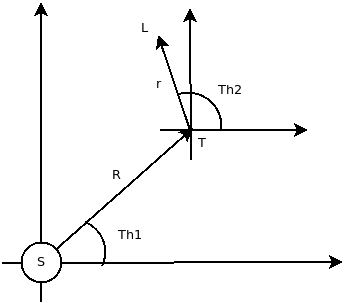
\includegraphics[width=\textwidth]{\fig/ex_sun_earth_moon.png}
\end{column}
\end{columns}
Allo stesso modo, rispetto ad un sistema di riferimento che si muove con il
pianeta, il moto del satellite, prendendo $r$ come raggio della circonferenza e
$T_L$ periodo di rivoluzione:
\begin{displaymath}
\mathcal{C}_{LT}:\begin{cases}
 x(t)= r \mcos(\frac{2\pi~t}{T_L})\\
 y(t)= r \msin(\frac{2\pi~t}{T_L})\\
 z(t)= 0
\end{cases}
\end{displaymath}
\end{frame}
\begin{frame}
\frametitle{Scrittura delle equazioni}

\begin{columns}
\begin{column}{0.5\textwidth}
Questo ci permette di scrivere l'equazione per il satellite nel sistema di riferimento della stella come la posizione del pianeta rispetto alla stella  pi\`u la posizione del satellite rispetto al pianeta:
\end{column}
\begin{column}{0.5\textwidth}
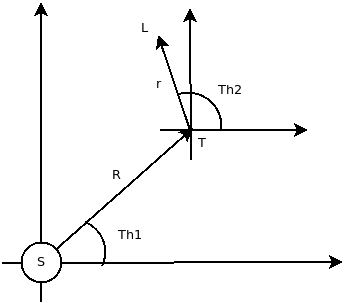
\includegraphics[width=\textwidth]{\fig/ex_sun_earth_moon.png}
\end{column}
\end{columns}
\begin{displaymath}
\mathcal{C}_{LS}:\begin{cases}
 x(t)=  R \mcos(\frac{2\pi~t}{T_T}) + r \mcos(\frac{2\pi~t}{T_L})\\
 y(t)=  R \msin(\frac{2\pi~t}{T_T}) + r \msin(\frac{2\pi~t}{T_L})\\
 z(t)= 0
\end{cases}
\end{displaymath}
\end{frame}
\begin{frame}
\frametitle{Fissare i parametri} 
Con le equazioni per $\mathcal{C}_{TS}$ e $\mathcal{C}_{LS}$, non rimane che
decidere la lunghezza dei due raggi (per i quali, per ottenere un risultato
realistico, vorremmo $r<R$), ed i due periodi $T_T$ e $T_L$.  

\begin{itemize}
\item Nel caso $T_T/T_S$ dia un risultato intero o frazionario, otterremo
un'orbita per il satellite che ad un certo punto si chiude e ricomincia il
ciclo da zero. Nella figura mostrata nel seguito si \`e scelto un $T_T/T_S =
12$ e le orbite del satellite si chiudono dopo un solo periodo di rivoluzione
del pianeta.  
\item In altri casi, l'orbita del satellite resta aperta e non si
ripete mai lungo lo stesso percorso. Il caso del sistema terra luna rientra sostanzialmente in questa categoria, con il periodo di rivoluzione terrestre di 365.25 giorni e quello lunare di circa 28 giorni. (Visualizzabile con \frnzplt fissando $T_T =1$, $T_L = 28/365.25$)
\end{itemize}
\end{frame}

\begin{frame}
\frametitle{}

\begin{columns}
\begin{column}{0.5\textwidth}
Caso $T_T = 1$, $T_L = 1/12$:
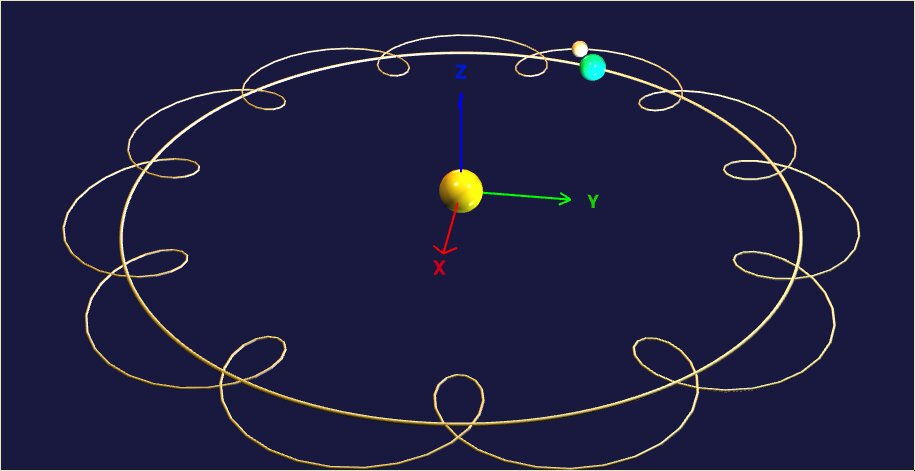
\includegraphics[width=\textwidth]{\fig/sunsys.jpeg}
\end{column}
\begin{column}{0.5\textwidth}
Caso $T_T = 1$, $T_L = 27/365.25$:
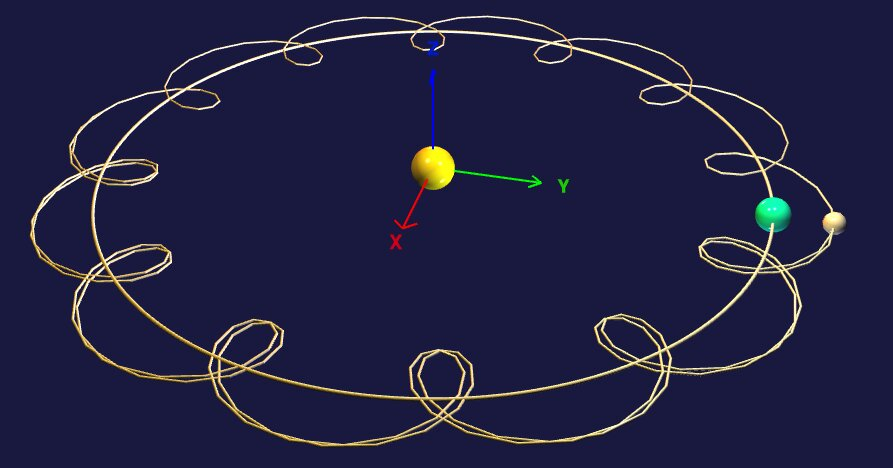
\includegraphics[width=\textwidth]{\fig/sunsys_real.jpeg}
\end{column}
\end{columns}
\end{frame}


\begin{frame}
\frametitle{Esercizio 5}

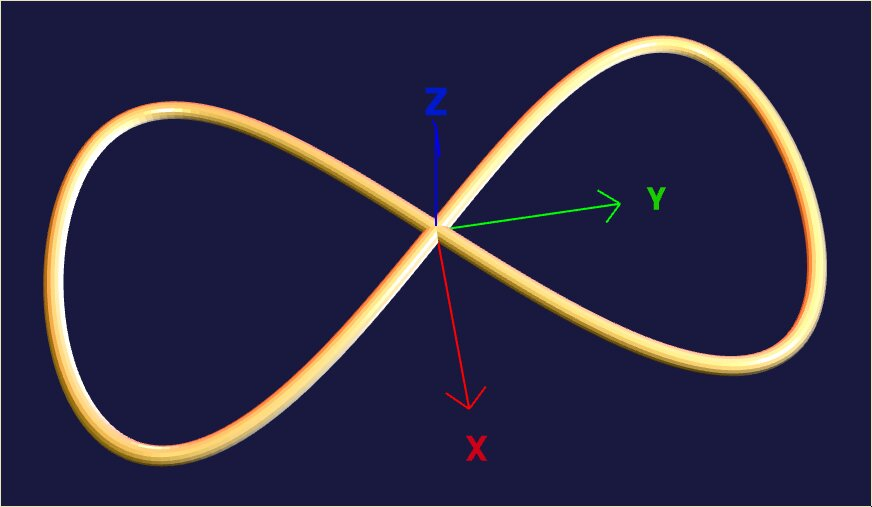
\includegraphics[width=0.8\textwidth]{\fig/infty.jpeg}

Determinare la forma della equazione parametrica che descrive questa curva. 
\end{frame}
\begin{frame}
\frametitle{Soluzione}
L'equazione di partenza e' quella di un'ellisse:
\begin{displaymath}
\mathcal{E}:\begin{cases}
 x(t)=  a \msin(t)\\
 y(t)=  b \mcos(t) & 0\leq t \leq 2\pi\\
 z(t)= 0
\end{cases}
\end{displaymath}
Si richiede alla coordinata $x$ di tornare al 0 quando la coordinata $y$
diventa 0. Confrontando i grafici di seno e coseno, si vede che \`e
sufficientemente cambiare $\msin(t)\rightarrow \msin(2~t)$.
\end{frame}
\begin{frame}
\frametitle{Soluzione - ii}
\begin{center}
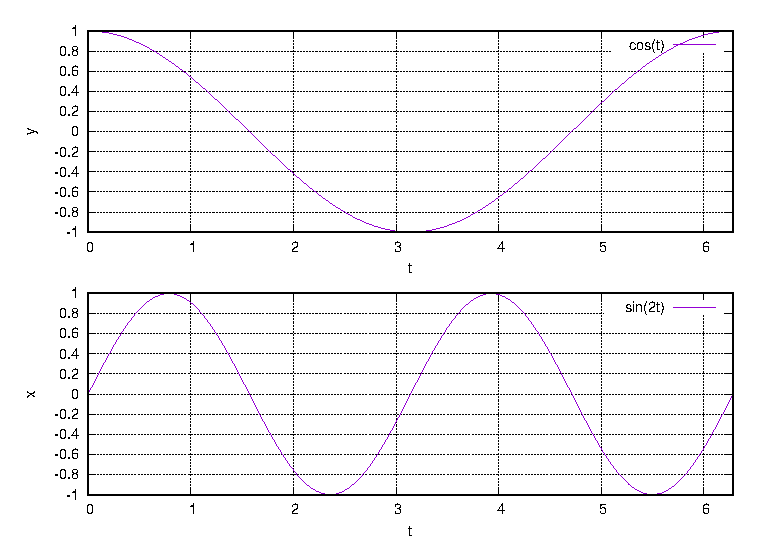
\includegraphics[width=0.6\textwidth]{\fig/es5_sol.eps}
\end{center}

\begin{displaymath}
\mathcal{E}:\begin{cases}
 x(t)=  a \msin(2t)\\
 y(t)=  b \mcos(t) & 0\leq t \leq 2\pi\\
 z(t)= 0
\end{cases}
\end{displaymath}
\end{frame}


\end{document}
